\section{研究方法}
\subsection{耗散粒子动力学}
\frame{ \frametitle{耗散粒子动力学简介}
\note{\textcolor{red}{[100-130s]}下面简要介绍一下耗散粒子动力学:}
  \begin{itemize}
  \item 耗散粒子动力学(DPD)是一种粗粒化的分子动力学方法,适合模拟介观尺度的简单和复杂流体动力学和流变性能.
        \note[item]{耗散粒子动力学(DPD)是一种粗粒化的分子动力学方法}
  \item 由Hoogerbrugge与Koelman首先提出, 旨在解决经典分子动力学难以解决的流体
        时间和空间尺度问题.
        \note[item]{提出这一方法的目的是为了解决经典分子动力学难以解决的流体时间和空间尺度问题}
  \item 优点: 与经典分子动力学方法相比, DPD方法可以使用更大的粒子尺寸和更长的时间步长, 因此具有更好的计算效率与计算能力,能应用到介观尺度乃至亚宏观的问题.
        \note[item]{因此相对于经典分子动力学, DPD由于可以使用更大的粒子尺寸和更长的时间步长,而且有更好的计算效率与计算能力.}
  \item 应用: 各类复杂的流体流动, 如相分离, 蛋白质等大分子悬浮, 表面活性剂, 胶
        体输运, 稀释聚合物溶液, 生物薄膜, 以及介观尺度的多相流动现象.
        \note[item]{现在的应用也相当广泛.}
  \end{itemize}
}

\frame{\frametitle{运动方程}
\begin{columns}
\begin{column}[c]{0.35\textwidth}
\begin{center}
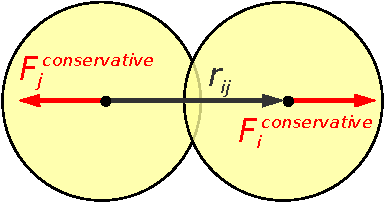
\includegraphics[width=0.9\textwidth]{conservative.pdf}
\vspace{1em}

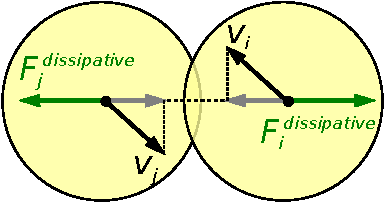
\includegraphics[width=0.9\textwidth]{dissipative.pdf}
\vspace{1em}

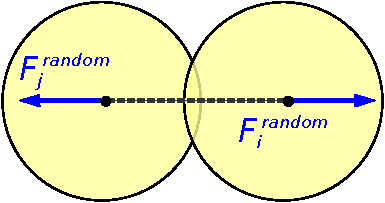
\includegraphics[width=0.9\textwidth]{random.pdf}
\end{center}
\end{column}
\begin{column}[c]{0.65\textwidth}
\note{\textcolor{red}{[130-145s]}}
牛顿运动方程描述DPD粒子运动\note[item]{DPD模型中粒子的运动由牛顿运动方程描述.}
  \[
  \frac{d\mathbf{r}_i}{dt} = \mathbf{v}_i,   
  \frac{d\mathbf{v}_i}{dt} = \mathbf{f}_i = \mathbf{f}_i^{\text{int}} + \mathbf{f}_i^{\text{ext}}
  \]
\note[item]{耗散粒子动力学中的粒子除了受到保守力外, 还受到耗散力和随机力.}
%\note[item]{耗散力方向与粒子间相对运动的方向相反, 因此通常会减弱粒子间相互作用, 减少系统的动能, 降低系统的温度.}
%\note[item]{而随机力则通常引起粒子间的随机振动, 增加系统的动能, 提高系统的温度.}
%\note[item]{耗散力和随机力的相互作用, 在满足一定条件下, 能使整个系统温度维持在基本恒定的水平上.}
DPD粒子间作用力包括保守力, 耗散力及随机力:
  \[
  \textcolor{red}{\mathbf{F}_{ij}^C = a_{ij}w^C(r_{ij})\mathbf{\hat{r}}_{ij}}
  \]
  \[
  \textcolor{MyDarkGreen}{\mathbf{F}_{ij}^D = -\gamma w^D(r_{ij})\Big(\mathbf{\hat{r}}_{ij}\cdot \mathbf{v}_{ij}\Big)\mathbf{\hat{r}}_{ij}}
  \]
  \[
  \textcolor{blue}{\mathbf{F}_{ij}^R = \sigma w^R(r_{ij})\xi_{ij}\mathbf{\hat{r}}_{ij}}
  \]
保守力权函数$w^C(r_{ij})$, 一般取为$1-r_{ij}$.
\end{column}
\end{columns}
}


\subsection{珠簧链模型}

\frame{\frametitle{珠簧链模型}
\begin{columns}
\begin{column}[c]{0.5\textwidth}
\begin{figure}
\centering
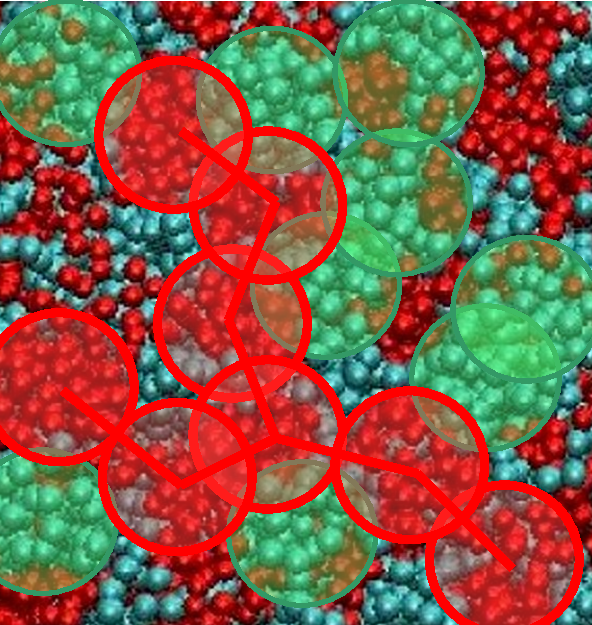
\includegraphics[width=\textwidth]{polymer.pdf}
\end{figure}
\end{column}
\begin{column}[c]{0.5\textwidth}
\note{\textcolor{red}{[145-165s]} 在DPD方法中, 模拟高分子时常用珠簧链模型, 把高分子链抽象成由弹簧力连接的DPD粒子. 下面是三种常用的珠簧链模型.}
\begin{itemize}
\item 简谐珠-簧链模型
\[
U_{\text{harmonic}} = \frac{k_s}{2}(l-l_0)^2
\]
\item FENE珠-簧链模型
\[
U_{\text{FENE}} = -\frac{k_s}{2}l_m^2\log(1-x^2)
\]
\item WLC珠-簧链模型
\[
U_{\text{WLC}} = \frac{k_B T l_m}{4p}\frac{3x^2-2x^3}{1-x}
\]
\end{itemize}
\end{column}
\end{columns}
}
